\documentclass{standalone}
\usepackage{tikz}
\usepackage{amsmath}
\usepackage{amsfonts}
\usepackage{amssymb}
\usepackage{pgfplots}

\pgfplotsset{compat=newest}
\begin{document}
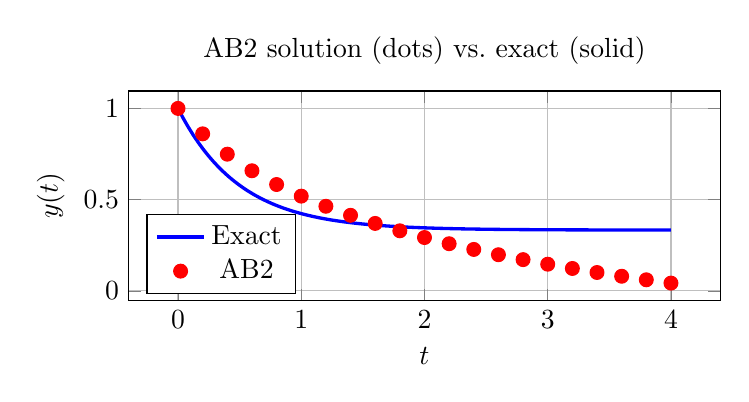
\begin{tikzpicture}
    \begin{axis}[
            width=0.75\textwidth,
            height=0.35\textwidth,
            xlabel={$t$}, ylabel={$y(t)$},
            title={AB2 solution (dots) vs.\ exact (solid)},
            legend pos=south west,
            grid=both
        ]
        \addplot[domain=0:4, samples=100, very thick, color=blue] {(2*exp(-2*x)+1)/3};
        \addlegendentry{Exact}
        \addplot[only marks, mark=*, mark size=2.5pt, color=red]
        coordinates {
                (0.0, 1.0000)
                (0.2, 0.8607)
                (0.4, 0.7492)
                (0.6, 0.6583)
                (0.8, 0.5830)
                (1.0, 0.5192)
                (1.2, 0.4637)
                (1.4, 0.4142)
                (1.6, 0.3697)
                (1.8, 0.3293)
                (2.0, 0.2924)
                (2.2, 0.2585)
                (2.4, 0.2272)
                (2.6, 0.1982)
                (2.8, 0.1713)
                (3.0, 0.1462)
                (3.2, 0.1228)
                (3.4, 0.1008)
                (3.6, 0.0802)
                (3.8, 0.0608)
                (4.0, 0.0426)
            };
        \addlegendentry{AB2}
    \end{axis}
\end{tikzpicture}
\end{document}